\Name{卞卓航}
\vspace{0em}
\Subtitle{北京大学 | 集成电路学院 | 电子设计自动化与计算系统}
\vspace{0.06em}

\noindent\begin{tabularx}{\linewidth}{@{}>{\raggedright\arraybackslash}X@{\hspace{0.55em}}>{\raggedleft\arraybackslash}p{2.45cm}@{}}
\begin{minipage}[t]{\linewidth}
\vspace{0pt}
\SectionBar{基本信息}
\BodyLine{男 \quad 22岁 \quad 汉族 \quad 中共党员 \quad 江苏无锡}
\BodyLine{电话/微信：13656160098 \hspace{5em} 邮箱：\underline{\href{mailto:bianzhuohang26@stu.pku.edu.cn}{bianzhuohang26@stu.pku.edu.cn}}}
\BoldLine{本科：北京航空航天大学 - 计算机学院 - 计算机科学与技术（2022--2026）}
\BoldLine{直博：北京大学 - 集成电路学院 - 电子设计自动化与计算系统（2026--）}
\end{minipage}
&
\vspace*{-2em}
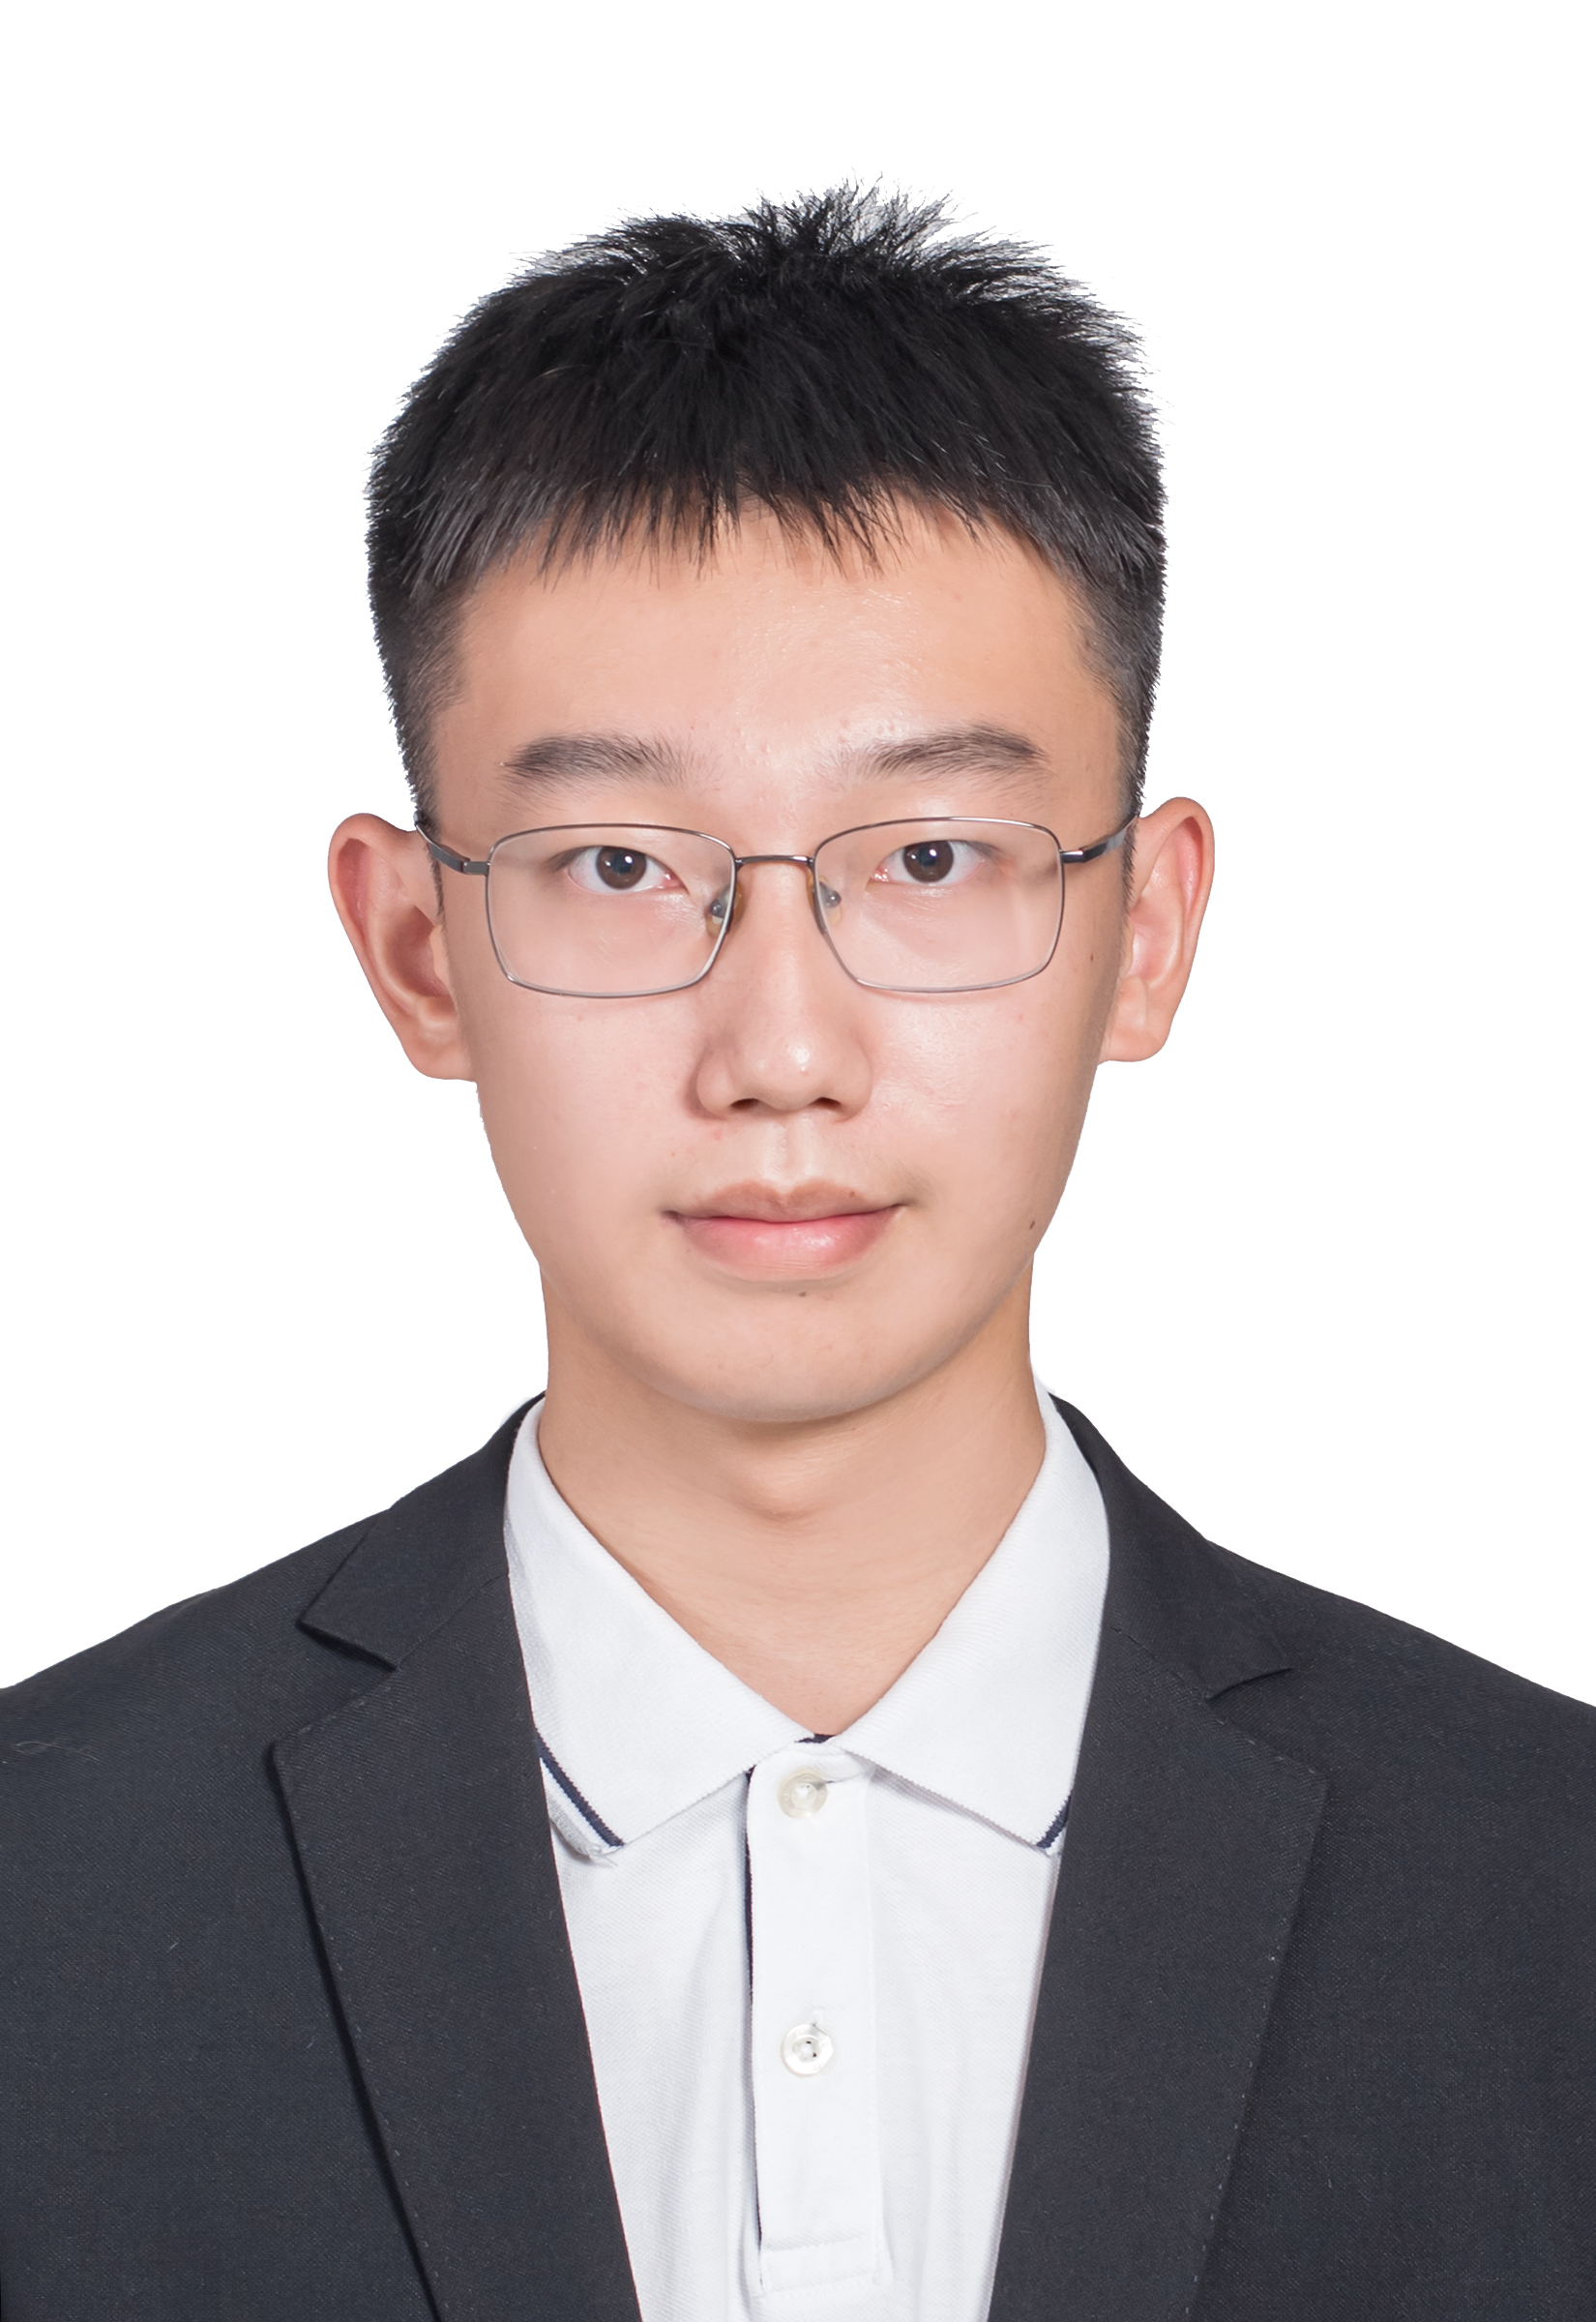
\includegraphics[width=2.36cm]{assets/headshot.jpg}
\end{tabularx}

\SectionBar{个人简述}
\BodyLine{聚焦 LLM 推理系统与体系结构，当前主要研究多智能体应用中的 KV Cache 管理与调度，具备从工作负载分析、系统设计到框架实现与评测的跨栈能力。}
\BulletLine{\textbf{本科专业排名 19/239（前10\%）；均分 92.54，GPA 3.86/4}}
\BulletLine{\textbf{核心专业课程成绩（部分）：} 面向对象100，智能计算体系结构99，概率统计99，数据挖掘97，计算机组成95\ldots}
\BulletLine{担任北航计算机学院\textbf{计算机组成课程高阶助教、操作系统课程助教}；\uline{\href{https://github.com/zhhangBian/Compiler-Techniques}{编译课程大作业}}为\textbf{全国教师培训实例代码}}

\SectionBar{科研经历}
\ResearchFocus{主要研究方向：多智能体 LLM 推理系统}{北大集成电路学院 · 卓有为助理教授团队 · 2025.2--至今}

\ProjectTitle{\uline{\href{https://arxiv.org/abs/2510.18586}{TokenCake}}：面向多智能体应用的 KV Cache 调度}{第一作者 · EuroSys 2027}
\BulletLine{针对 Function Call 场景中 KV Cache 的\textbf{时间空转}与多 Agent 并发带来的\textbf{空间争用}，抽象应用内部依赖与工具调用，识别关键路径缓存被非关键任务挤占的问题。}
\BulletLine{设计 agent-aware 的 \textbf{Time/Space Scheduler}，结合主动 offload、predictive upload 与动态内存分区；端到端时延较 vLLM 降低 \textbf{47.06\%}，有效 GPU KV Cache 利用率提升 \textbf{16.9\%}。}

\ProjectTitle{\uline{\href{https://arxiv.org/abs/2604.03143}{TokenDance}}：多智能体 KV Cache 集体复用与压缩}{第一作者 · Preprint}
\BulletLine{面向同步多轮交互中的 All-Gather 模式，发现共享输出在不同 Agent 上因位置偏移而无法被请求级前缀缓存有效复用，导致重复计算与显存冗余。}
\BulletLine{设计 \textbf{KV Collector} 与 \textbf{Diff-Aware Storage}，实现轮级 collective KV 复用和 block-sparse 差分存储；典型负载压缩 \textbf{11--17$\times$}，并发 Agent 数提升 \textbf{2.7$\times$}，prefill 加速 \textbf{1.9$\times$}。}

\ProjectTitle{\uline{\href{https://arxiv.org/abs/2503.08415}{TokenSim}}：LLM 推理系统软硬件联合模拟器}{第二作者 · APPT 2025}
\BulletLine{参与构建面向动态真实工作负载的模块化模拟器，支持可扩展的\textbf{调度器、内存管理器与算子级性能建模}，输出时延分布和随时间变化的显存占用。}
\BulletLine{基于真实系统验证仿真误差\textbf{低于 1\%}；支撑 PD 分离、异构硬件选择、显存配额与长对话内存池等软硬件设计空间探索。}

\vspace{0.5em}

\EntryTitle{
北航复杂关键软件环境全国重点实验室 \quad
刘祥龙教授团队 \quad
强化学习安全方向
}{2024.7-2025.1}

\BulletLine{搭建多智能体强化学习鲁棒性评测平台\textbf{AMB}，覆盖\textbf{4 个真实环境、13 类不确定性、15 项关键超参}，支撑 \textbf{82,620} 组实验。仅通过超参优化即可平均提升 cooperation \textbf{52.60\%}、robustness \textbf{34.78\%}、resilience \textbf{60.34\%}。}
\BulletLine{负责参与攻击算法与实验流水线实现、参与结果分析及论文撰写，围绕 cooperation / resilience 的关系展开研究；}
\BulletLine{NeurIPS 2025论文：\underline{\href{https://arxiv.org/abs/2510.11824}{arXiv:2510.11824}}}

\newpage

\EntryTitle{
北航中德联合软件研究所 \quad
栾钟治副教授团队 \quad
高性能计算方向
}{2023.9-2024.5}

\BulletLine{面向新一代天河超算上的 \textbf{MT-3000 CPU-DSP 异构处理器}，在 PyTorch 框架下优化 Multi-Head Attention；围绕 \textbf{Linear / Softmax} 等核心算子实现 DSP 定制化优化，并结合矩阵分块、DMA 双缓冲、通信优化与 head 级算子调度提升执行效率。}
\BulletLine{负责进行相应的算子注册实现（Pytorch1.8 C++ Extension），并在 MT-3000 上进行性能调优与评测；完成 Linear 算子实现。}
\BulletLine{HPC-CHINA 2024优秀论文：MT-3000 处理器上的 Multi-Head Attention 优化}

\SectionBar{项目经历}
\EntryTitle{「商汤科技实习」 \uline{\href{https://github.com/ModelTC/LightLLM}{LightLLM}} LLM推理加速框架算法研究}{2025.6-2025.10}
\BodyLine{在 \uline{LightLLM} 上进行 LLM 推理系统算法与框架开发，累计合入 \textbf{6 个公开 PR}，工作聚焦 \textbf{PD 分离调度、KV Cache 迁移与多模态模型适配}。}
\BulletLine{重构 PD Master 的节点选择链路，设计可扩展 selector 机制，并新增基于节点负载预测的\textbf{内存感知路由}与 load info 回传，用于缓解 Prefill / Decode 负载不均。}
\BulletLine{扩展 P/D 分离下的 KV Cache 迁移：为 chunked decode 增加\textbf{超时重试与 KV 回传}机制，并在多 DP 场景实现基于 \textbf{CUDA/NCCL} 的 kv\_trans\_v2 跨卡迁移。}
\BulletLine{适配 \textbf{MinerU2} 多模态模型到 LightLLM，打通 tokenizer、image processor、vision tower / projector、visual RPC 与服务端接口，并补充 token usage 与 server id 等可观测性能力。}
\BulletLine{相关链接：仓库 \underline{\href{https://github.com/ModelTC/LightLLM}{LightLLM}}；PR \underline{\href{https://github.com/ModelTC/LightLLM/pull/944}{\#944}} / \underline{\href{https://github.com/ModelTC/LightLLM/pull/970}{\#970}} / \underline{\href{https://github.com/ModelTC/LightLLM/pull/999}{\#999}} / \underline{\href{https://github.com/ModelTC/LightLLM/pull/1011}{\#1011}} / \underline{\href{https://github.com/ModelTC/LightLLM/pull/1024}{\#1024}} / \underline{\href{https://github.com/ModelTC/LightLLM/pull/1034}{\#1034}}}

\EntryTitle{2024年计算机系统能力大赛CPU赛道（龙芯杯）全国第四（二等奖）}{2024.7-2024.8}
\BulletLine{实现支持 LoongArch32R（除浮点外）的 \textbf{13 级乱序双发超标量处理器}，集成分支预测、L1 Cache、TLB，可启动 Linux；FPGA 频率达 \textbf{80MHz}，平均 IPC \textbf{1.02}，获全国第四（二等奖）。}
\BulletLine{4 人团队中负责后端关键模块与联调，重点实现 \textbf{ALU/LSU/MDU Issue Queue、Commit/访存状态机} 等逻辑。}
\BulletLine{仓库链接：\underline{\href{https://github.com/zhhangBian/BOOM_chip}{https://github.com/zhhangBian/BOOM\_chip}}}

\SectionBar{荣誉奖项}
\AwardItem{\textbf{北京市优秀毕业生}（2026）}
\AwardItem{全国大学生数学建模竞赛\textbf{全国一等奖}（2024）}
\AwardItem{全国大学生计算机系统能力大赛\textbf{全国二等奖}（2025）}
\AwardItem{计算机系统能力大赛 CPU 赛道（龙芯杯）\textbf{全国第四/二等奖}（2024）}
\AwardItem{美国大学生数学建模竞赛\textbf{一等奖/Meritorious Winner}（2024）}
\AwardItem{北京市大学生物理竞赛\textbf{一等奖}（2023）}
\AwardItem{\textbf{航空工业奖学金}、“七三奖章”奖学金}
\AwardItem{北航学习优秀一等奖、竞赛特等奖、创新创业二等奖}
\AwardItem{北航\textbf{优秀学生干部}（2023--2025）、优秀团干部、优秀学生}

\SectionBar{语言与技能}
\BodyLine{语言：\textbf{CET-6：589}}
\BodyLine{个人博客： \underline{\href{https://zhhangbian.github.io/}{https://zhhangbian.github.io/}}}
\BodyLine{技术：\textbf{Python / C++ / CUDA / SystemVerilog}；熟悉 LLM Serving、分布式推理、处理器设计与强化学习实验平台开发。}
\BodyLine{工程：负责\textbf{北航计算机组成课程教学系统}运行维护；具备 Linux 运维、前后端开发与实验平台搭建经验。}
